\documentclass{article}
\usepackage{setspace}   %Allows double spacing with the \doublespacing command
\usepackage{lipsum} % Add dummy text
\usepackage{graphicx}
\begin{document}

\title{Population prediction based on satellite imagery\\
Term Project Report} 

\date{December 2017}
\author{Yassine Kadiri, Santiago Novoa, Zsolt Pajor-Gyulai, Manuel Serrano}
\maketitle

\doublespacing


\section{Summary}
In this project, we attempted to build models predicting population density based on satellite imagery inspired by \cite{RHD17}. We achieve this by comparing spatially disaggregated census data on the continental United States (that is excluding Alaska and U.S. territories) to satellite images of the particular region. We use several approaches: 
\begin{itemize}
\item[(1)] naive logistic regression on the vectorized satellite images; 
\item[(2)] convolutional neural network(CNN) built from scratch; \item[(3)] pre-trained CNN developed for image recognition (Vgg16).
\end{itemize}

While our models do not achieve particularly high accuracy, they show considerable lift corresponding to random guessing. Perhaps not surprisingly, the pre-trained neural network showed the best performance of achieving $62\%$ accuracy. [Finish this with final conclusions]

\section{Business understanding}
The 'business' in question in this case is mostly non-profit, governmental application. In order to allocate resources, government agencies require knowledge on the geographical distribution of the country's population. In the absence of direct measurements in years between two censuses, these entities are forced to rely on ad-hoc methods to model the evolution of the population since the last census year (\cite{L96}).

Our project explores the possibility of obtaining direct measurements of the population of a particular area by looking at Satellite imagery. Such capability would be of great value in many decision making processes such as urban development, evacuation planning, and gauging future demand for food, water, energy, and services. For example, according to the US General Accounting Office, more than 70 federal programs distribute tens of billions of dollars annually on the basis of population estimates.

Furthermore, censuses in many countries are non-representative due to limited civil registration systems or are outright fraudulent (\cite{BDYPHN06}). In this case, having an independent way to estimate population could be beneficial in the optimal allocation of humanitarian aid or for clandestine purposes.

\section{Data}
\subsection{Data understanding}

\subsection{Data preparation}
\section{Modeling and evaluation}
Our goal in this section is to show that we can extract predictive value from our data, that is, our models provide a non-unit lift compared to random guessing.
\subsection{Logistic regression}
\subsection{CNN from scratch}
\subsection{Pretrained VGG architecture}
The Vgg16 architecture is a 16 layer CNN developed for large scale image recognition by the Visual Geometry Group at the University of Oxford (\cite{SZ14}). This architecture won the ILSVRC-2014 ImageNet competition in 2014. We use the Keras version that has been obtained by directly converting the Caffe model provided by the authors\footnote{https://gist.github.com/baraldilorenzo/07d7802847aaad0a35d3, however, we use the modified version adapted to the Fast.ai course.}.

We used this CNN to perform multi-type classification with respect to eight population intervals:
\begin{figure}[ht]
\center
\begin{tabular}{ |c|c| } 
\hline
Population interval & Number of images\\
\hline
0-1& 154\\ 
1-10& 782\\ 
10-50& 2813\\
50-100& 908\\
100- 500& 1294\\
500-1000& 529\\
1000-2000& 401\\
2000-11000& 119\\
Total& 7000\\
\hline
\end{tabular}
\caption{Population intervals and the number of corresponding images in our dataset of images. The upper end of the intervals is inclusive, while the lower end is excluded, except for the very first interval.}
\end{figure}

Vgg16 is designed to assign probability scores of an image belonging to 1000 different ImageNet categories. We finetune the network according to our population intervals, that is we use the ImageNet scores as features to predict our population intervals (so essentially we assign scores that a satellite image is a dog, cat, corn, ketchup, etc. and then use these scores as inputs for classification). After performing a random $80\%-20\%$ split between the training and validation set, we performed 30 training epochs using the ADAM\footnote{https://machinelearningmastery.com/adam-optimization-algorithm-for-deep-learning/} algorithm with learning rate $0.001$ and categorical cross-entropy as our loss function. This gave us validation accuracy of $62\%$ and validation loss $1.0054$. Moreover the confusion matrix on the validation set is:
\begin{figure}[ht]
\centering
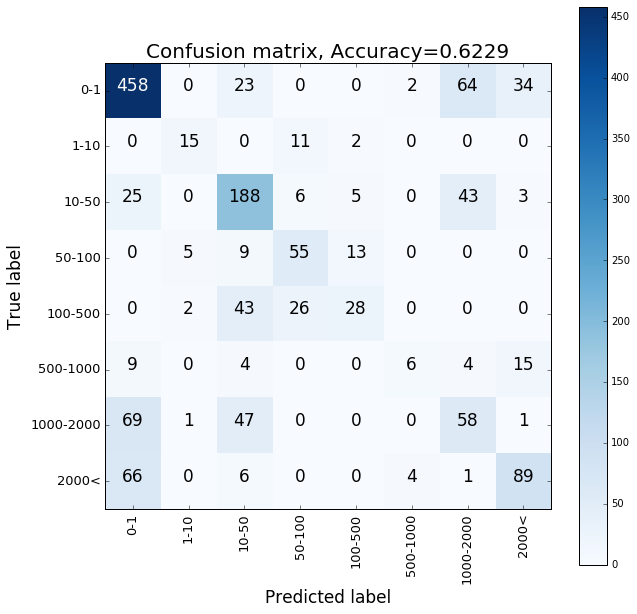
\includegraphics[scale=0.45]{conf_mx_Zsolt1.png}
\end{figure}

To see if we can improve performance, we also attempted to retrain the ImageNet layer of the model (using the finetuned model above, to avoid starting with random weights in the final layer, which would cause the retrained layer to quickly move a long way from its optimized ImageNet weights): This gave us  validation accuracy of $\%$ and the validation set confusion matrix:

\subsection{Comparison ?}
To compare the accuracy of our models on an independent test set, we considered a balanced set of images close to the area where our original sample was obtained. Since the set is balanced over the population intervals, the accuracy of random guessing is $1/8=12.5\%$.

[...]

To test our models on a different terrain, we obtain a small balanced test set from the San Francisco bay area.

[...]

\section{Deployment}
After a successful validation of our models, deployment should be in the form of an automated software implementation, where decision makers can obtain the figure on the population of a particular area by simply feeding the neural network the corresponding satellite images.

However, every governmental agency using our model for decision making should be aware of the imperfection of our predictions. Accordingly, whenever human life depends on the results (e.g. evacuation planning, or disaster relief funds), the policymakers should make sure to have appropriate cushion built into their actions. To provide further security, the cautious user should use our models in conjunction with other techniques and be alerted by huge discrepancies. This of course applies to all other applications with, perhaps, less severe consequences.

As features of areas populated by humans, in particular overall architecture, change rather slowly over time, one would expect a well trained model to be robust over a long period of time. Of course, the model should go through revalidation or, perhaps, retraining from time to time. A natural point for this to occur are the census years, when labeled data becomes available.

Unless it is the explicit goal of using the model (e.g. in clendestine applications), one has to be aware that obtaining satellite images of people's properties raises obvious privacy issues. The respectful user should use a low enough resolution such that the details of individual's properties cannot be extracted from the image.

\section{Possible further directions}

There are many interesting questions arising in connection with using our models that we did not have the chance to investigate due to the lack of time and data acquisition difficulties.

For example, we could have looked at different (preferrably larger) training sets containing different terrains, e.g., training in California and testing on the east coast. We could have also tried to perform population estimates on foreign countries to see how well our models generalize. For example, it would have been interesting to predict the population of North Korea and see how the measurement would correlate with the official figure. Finally, we could have used different population intervals to see if it increases accuracy.

\appendix
\section{Contribution of each team member to the project}
\subsection{Yassine Kadiri}
\subsection{Santiago Novoa}
\subsection{Zsolt Pajor-Gyulai}
Researched the paper \cite{RHD17}, when the project proposal came up. Worked on the write-up of the project proposal. Learned how to use the Vgg architecture (and how to do any sort of deep learning in the first place) from the online Fast.ai course. Built the Vgg model and wrote the corresponding section in this write-up. Wrote the first version of the 'Summary', 'Business understanding', and 'Deployment' sections of this write-up.
\subsection{Manuel Serrano}

\begin{thebibliography}{9}

\bibitem[BDYPHN06]{BDYPHN06} \textsc{D. Balk, U. Deichmann, G. Yetman, F. Pozzi, S. Hay, A. Nelson} \textit{ Determining global population distribution: methods, applications, and data.} Advances in parasitology, Vol 62, p119-156 (2006)

\bibitem[L96]{L96} \textsc{J. Long}\textit{ Postcensal population estimates: States counties and places.} Indirect Estimators in US Federal Programs, p59-82, Springer (1996)

\bibitem[RHD17]{RHD17}  \textsc{C. Robinson, F. Hohman, B. Dilkina}\textit{ A Deep Learning Approach for Population Estimation from Satellite Imagery.} arXiv preprint arXiv:1708.09086 (2017)

\bibitem[SZ14]{SZ14} \textsc{K. Simonyan, A. Zisserman} \textit{ Very Deep Convolutional Networks for Large-Scale Image Recognition} arXiv preprint arXiv:1409.1556
\end{thebibliography}
\end{document}